% 03_methods.tex (English)

This section details the Spectral-Temporal Transformer architecture and the training procedure.

\subsection{Problem Statement}
Given the Laplacian spectrum $(\Lambda,U)$ of graph $G$, our goal is to predict the FALQON parameter sequence $\bm{\beta}=(\beta_0,\ldots,\beta_{P-1})$, modeled as a conditional sequence generation problem:
\begin{equation}
 p(\bm{\beta}|G)=\prod_{t=0}^{P-1} p(\beta_t|\beta_{<t},G).
\end{equation}

\subsection{Model Architecture}
As shown in Figure \ref{fig:architecture}, the model consists of three modules.

\begin{figure}[htbp]
  \centering
  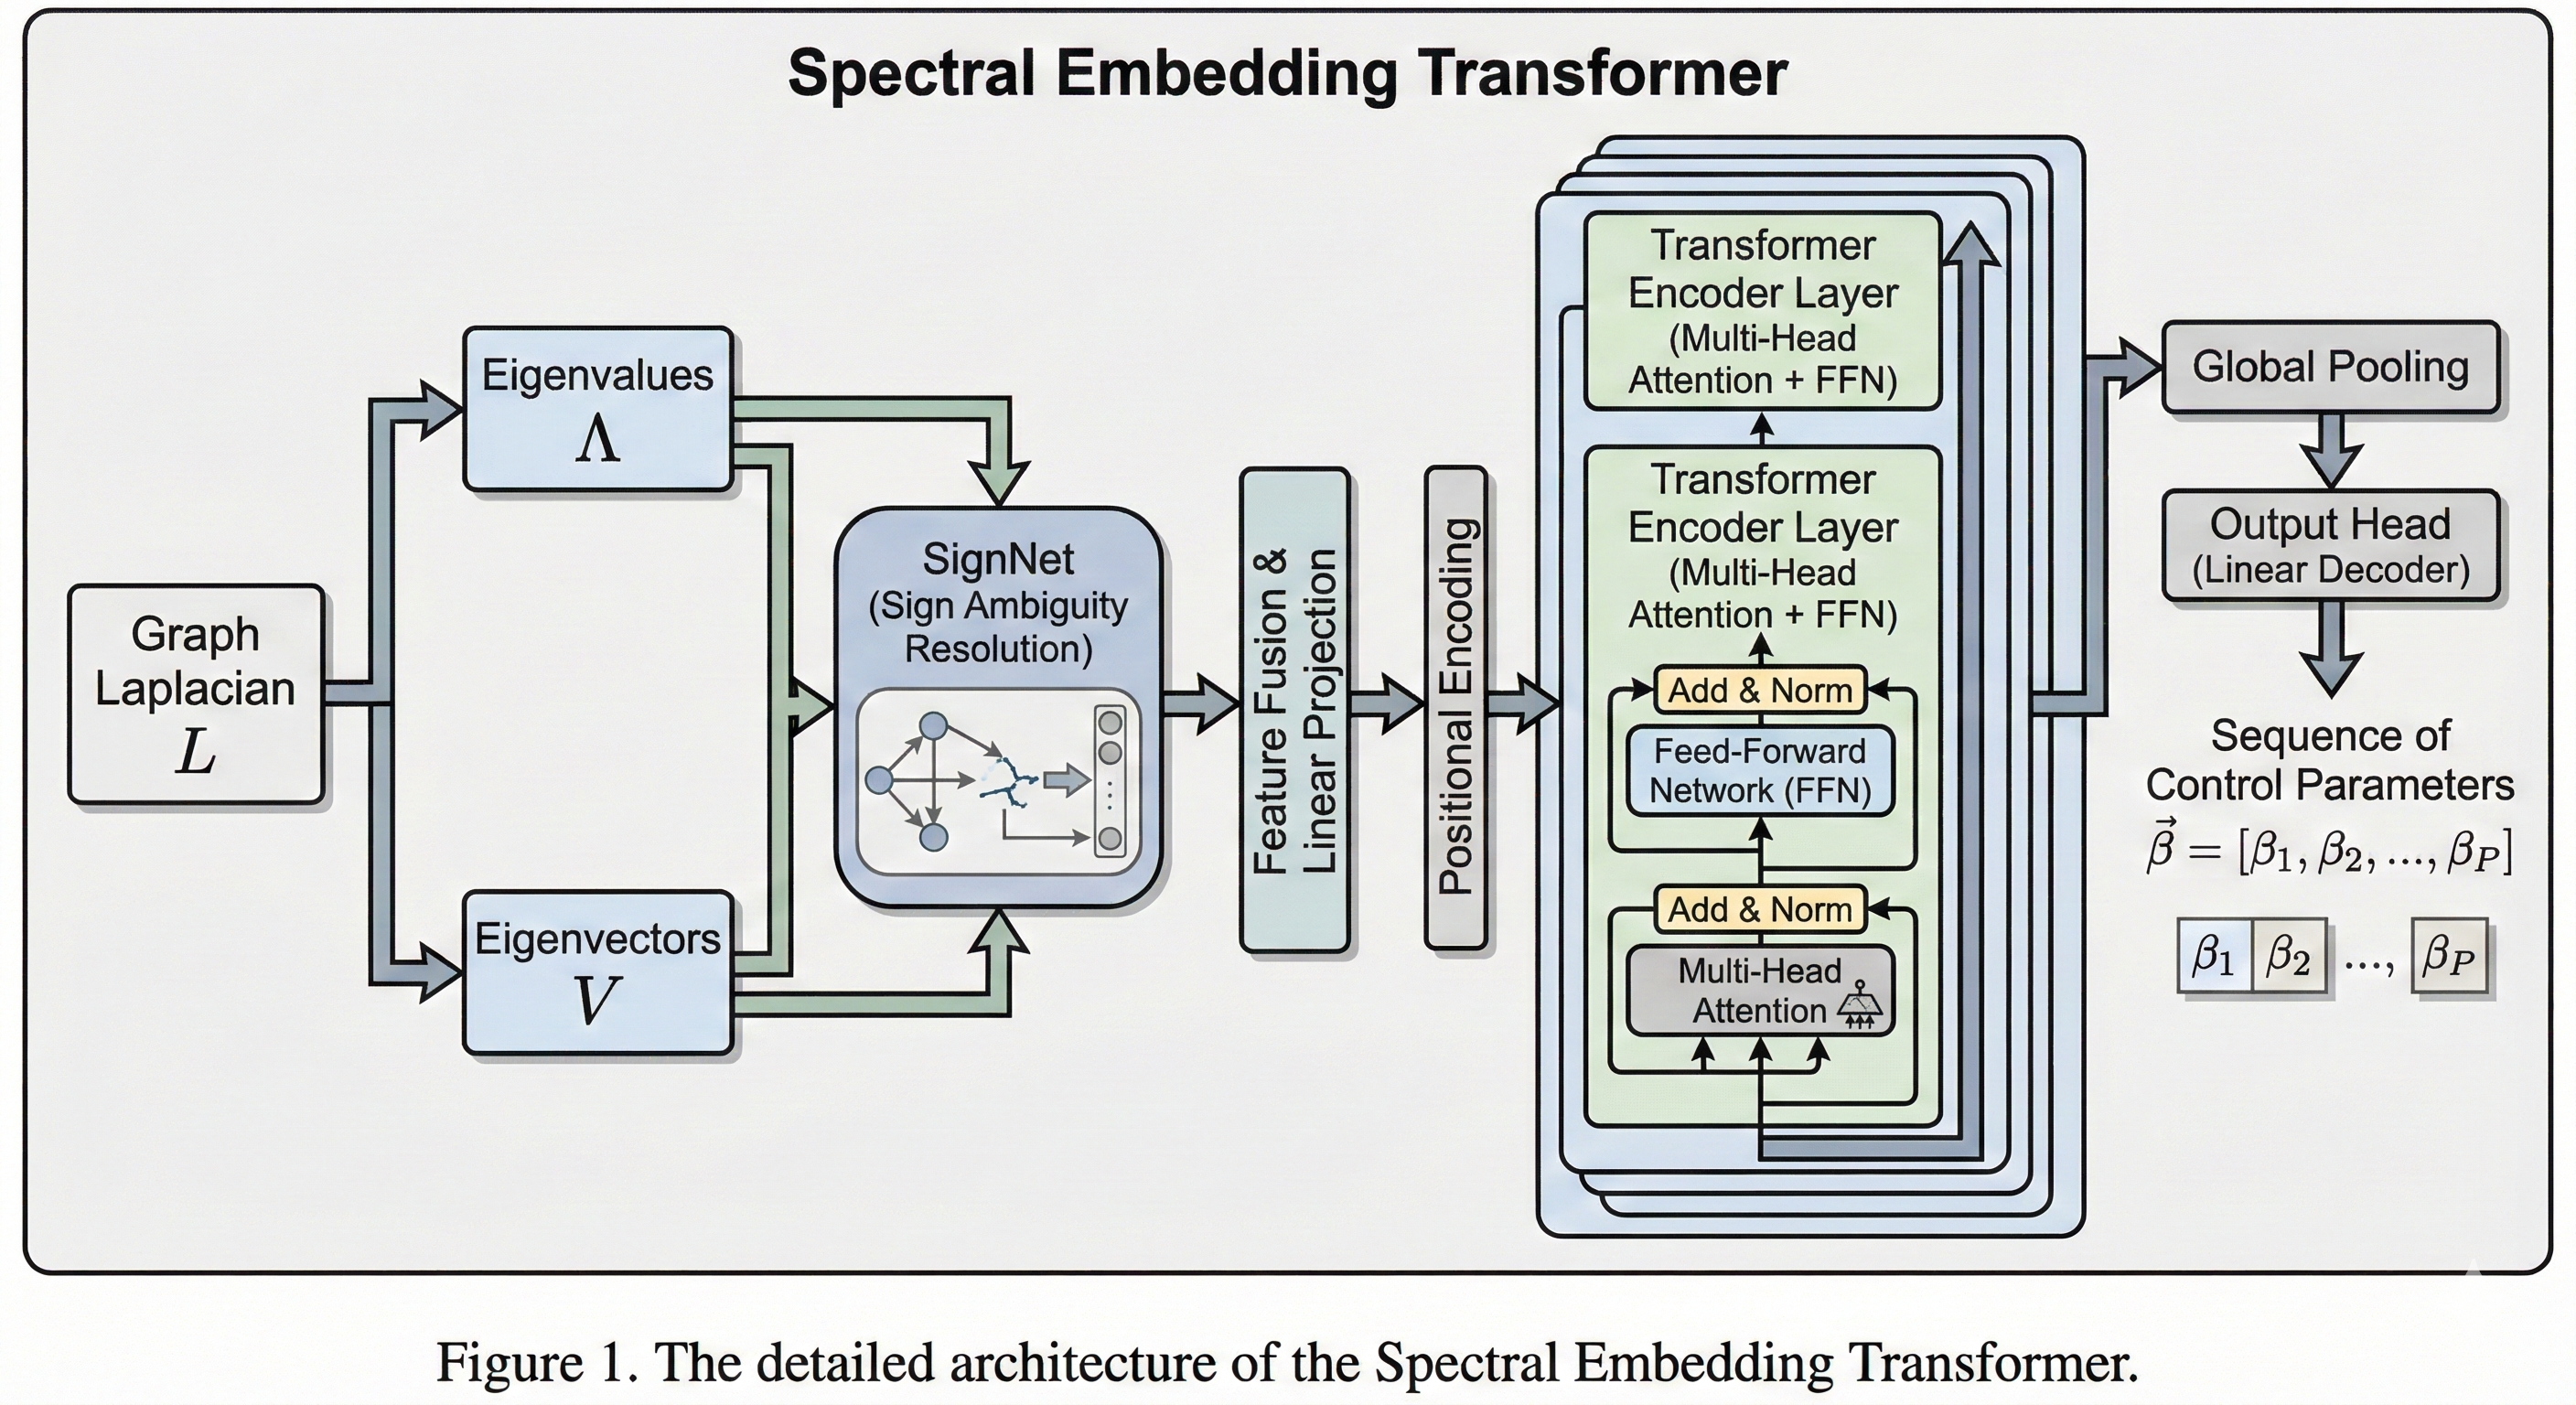
\includegraphics[width=0.9\linewidth]{../essay/figures/transformer_architecture.png}
  \caption{Overview of the Spectral-Temporal Transformer architecture.}
  \label{fig:architecture}
\end{figure}

\subsubsection{Sign-invariant Spectral Encoder (SignNet)}
\label{subsec:signnet}
We remove eigenvector sign ambiguity using a SignNet-style encoding:
\begin{equation}
 h_i=\rho(\phi(u_i)+\phi(-u_i)),
\end{equation}
where $\phi$ is an MLP and $\rho$ aggregates.

Eigenvalues are separately encoded and fused: $m_i=\mathrm{Fusion}(\mathrm{MLP}(\lambda_i),h_i)$, resulting in $M$ spectral modes used as memory for the decoder.

\subsubsection{Temporal Decoder}
We use a Transformer decoder \cite{vaswani2017attention} where queries are formed by positional encodings and previous-step embeddings:
\begin{equation}
 q_t=\mathrm{PE}(t)+\mathrm{Embed}(\beta_{t-1})+e_{\mathrm{query}}.
\end{equation}
Cross-attention queries the spectral memory to produce predictions.

\subsubsection{Output Head}
Decoder outputs are mapped to scalars: $\hat{\beta}_t=\mathrm{MLP}(\mathrm{Decoder}(q_t,M))$.

\subsection{Training}
We use scheduled sampling \cite{bengio2015scheduled} to bridge training and inference, and a loss combining weighted MSE, temporal-gradient loss and tail-variance regularization.
